\section{System}\label{System}

Delta is a DSL implemented as a React library for augmenting mathematical formulas and surrounding explanations with interactivity. Authors write a configuration that declares formulas as \LaTeX{} strings---the notation authors already know---variables as interactive symbols, a semantics function for computation, and visualizations that synchronize with the formula state. A \texttt{Provider} component abstracts away all MathJax setup and reactive update logic (Table~\ref{tab:mathjax-comparison}); authors place \texttt{Formula} and \texttt{Graph} components by \texttt{id} alongside prose and other content. Common interactive patterns require minimal configuration beyond the formula itself, while the specification is compositional---each addition extends what came before, so authors moving beyond defaults build on existing work rather than starting over.

\subsection{Substitution}

\paragraph{Input.} Delta supports the four interaction patterns identified by Head et al.~\cite{Head2022-ws} through three input mechanisms. \textit{In-formula input}: within the rendered formula, \texttt{drag} variables enable scrubbable expressions where readers click and drag on a value to change it in place, while \texttt{inline} variables replace symbols with editable text fields for direct entry. \textit{In-prose input}: \texttt{InlineVariable} components place the same draggable or editable controls within running text, functioning as external controls that influence formula values from outside the expression. \textit{Custom input}: authors create arbitrary input widgets---sliders, dropdowns, or domain-specific controls---via \texttt{Custom()} components that read and write values through the \texttt{vars} proxy (Table~\ref{tab:custom-api}). Linked selections emerge automatically: hovering over any variable highlights it across all \texttt{Formula}, \texttt{InlineVariable}, and \texttt{Custom} components sharing that identifier. A compact set of properties---\texttt{input}, \texttt{range}, \texttt{step}, \texttt{default}, \texttt{name}---allows rapid specification of essential presentation dimensions (Table~\ref{tab:variable-properties}). In a gradient descent walkthrough (Figure~\ref{fig:system}), an \texttt{InlineVariable} in the prose lets readers drag the label $y$---and dragging directly on the graph updates $y$ just the same.

\paragraph{Computation.} The \texttt{semantics} function provides expressiveness in computation: authors access variables by the same identifiers used in the formula---\texttt{vars.x} reads or writes \texttt{x}---then write plain JavaScript with full access to loops, conditionals, external libraries, and helper functions for complex calculations (Table~\ref{tab:vars-access}). When any input changes, Delta automatically re-executes the semantics function. Because the same function handles \texttt{step()} calls for walkthroughs and \texttt{sample()} calls for visualizations, a single computation pass updates all dependent data.

\subsection{Walkthroughs}

Delta supports walkthroughs that \textit{align sequencing with semantics}: the narrative structure of an explanation maps directly onto the computational structure of the formula. Within the semantics function, authors insert \texttt{step()} calls at meaningful points in the computation---after computing a gradient, before updating a weight---breaking the algorithm into discrete, narrated stages that mirror how the math actually unfolds. When \texttt{stepping: true} is set, the system presents navigation controls for stepping forward and backward, letting readers trace the same logical path the computation follows. This proves especially valuable for iterative algorithms like gradient descent, where each pass through the loop updates multiple interdependent quantities that readers must track together.

Each \texttt{step()} accepts a configuration object with two properties: \texttt{description} for narrated annotations and \texttt{labels} for positioning values on the formula. Descriptions support inline \LaTeX{} with \texttt{\$...\$} and string concatenation with computed variables from the semantics function---e.g., \texttt{`Error is \$\{vars.error\}\$`}---so annotations stay synchronized with the current state. Labels use \LaTeX{} substrings as selectors: keys matching variable identifiers (e.g., \texttt{w\_t}) attach values to those symbols, while keys matching longer expressions (e.g., \texttt{y - w\_t \textbackslash cdot x}) highlight and annotate entire subexpressions. This selector syntax leverages authors' existing \LaTeX{} knowledge---the same strings that define the formula also address its parts. Label values can be numbers, strings with inline \LaTeX{}, or formatting calls such as \texttt{latex()}, \texttt{precision()}, and \texttt{sigfig()} that mirror the display settings available on variables themselves (Table~\ref{tab:variable-properties}).

The gradient descent walkthrough (Figure~\ref{fig:system}) illustrates these constructs working together across multiple formulas. In the loss formula, labels display the current error value on the squared-error expression; in the update rule, separate labels show the gradient, current weight, and next weight at their respective positions. Because \texttt{step()} accepts a record keyed by formula \texttt{id}, authors specify which labels appear on which formula at each stage---the loss computation shows its intermediate values while the weight update shows its own, all advancing in lockstep as readers navigate the walkthrough.

\subsection{Synchronization}\label{Visualizations}

\paragraph{Variables.} A core principle underlies the system: \textit{variables are universal indices}. The same \LaTeX{} token that appears in the formula serves as the key that connects notation, interactivity, computation, and visualization under a single identifier. As a result, variables are defined apart from formulas in Delta. Separating variables from formulas also enables multi-formula systems driven by a single semantics function, reduces reliance on symbolic solvers, and gives authors flexibility to design custom computational flows. The same \texttt{vars} interface is used not just in \texttt{semantics}, but also in custom components.

\paragraph{Synchronized representations.} Delta synchronizes formulas with visualizations so that manipulating one representation updates the other, keeping formula and graph as synchronized representations of the same object. A \texttt{Provider} component abstracts away all MathJax setup and reactive update logic (Table~\ref{tab:mathjax-comparison}); authors place \texttt{Formula} and \texttt{Graph} components by \texttt{id} alongside prose and other content.

\paragraph{Sampling.} To populate a plot, the semantics function emits data with \texttt{sample(sampleId, \{x, y\})} or \texttt{sample(sampleId, \{x, y, z\})}, separating the mathematical relationship from sampling and rendering. In 2D, \texttt{lines} sample over a parameter variable's range via \texttt{parameter}, while \texttt{points} display the current state; both reference data through \texttt{sampleId}. The \texttt{interaction} property enables bidirectional manipulation---e.g., \texttt{interaction: ["horizontal-drag", "x"]} lets readers drag a point to change \texttt{x}. Points and vectors can also synchronize with step-through mode via \texttt{stepId}, optionally accumulating across steps with \texttt{persistence: true}. 3D plots extend the same model to surfaces and meshes, rendered with Plotly.js. Users can also access the same programmatic sampling helpers directly---\texttt{sample2DLine()}, \texttt{sample2DPoint()}, \texttt{sample3DLine()}, \texttt{sample3DPoint()}, and \texttt{sampleSurface()}---and Delta uses these same calls internally to implement the library's \texttt{Graph} component. The \texttt{graph2d} and \texttt{graph3d} arrays declare plots that react to formula state; because variables serve as universal indices, the same identifiers key both semantics and visualization data.

\paragraph{useStore.} For domain-specific needs, authors can register custom React components via \texttt{Custom()}, which injects a \texttt{vars} proxy for reading and writing variable values while preserving the reactive connection. Lower-level components can also access the surrounding reactive state through \texttt{useStore()}, the hook used by Delta's built-in components to read and write variables within the enclosing \texttt{Provider}. The \texttt{Graph} component renders a visualization by \texttt{id}, composing freely alongside \texttt{Formula} and other content.

\begin{figure*}[t]
\centering
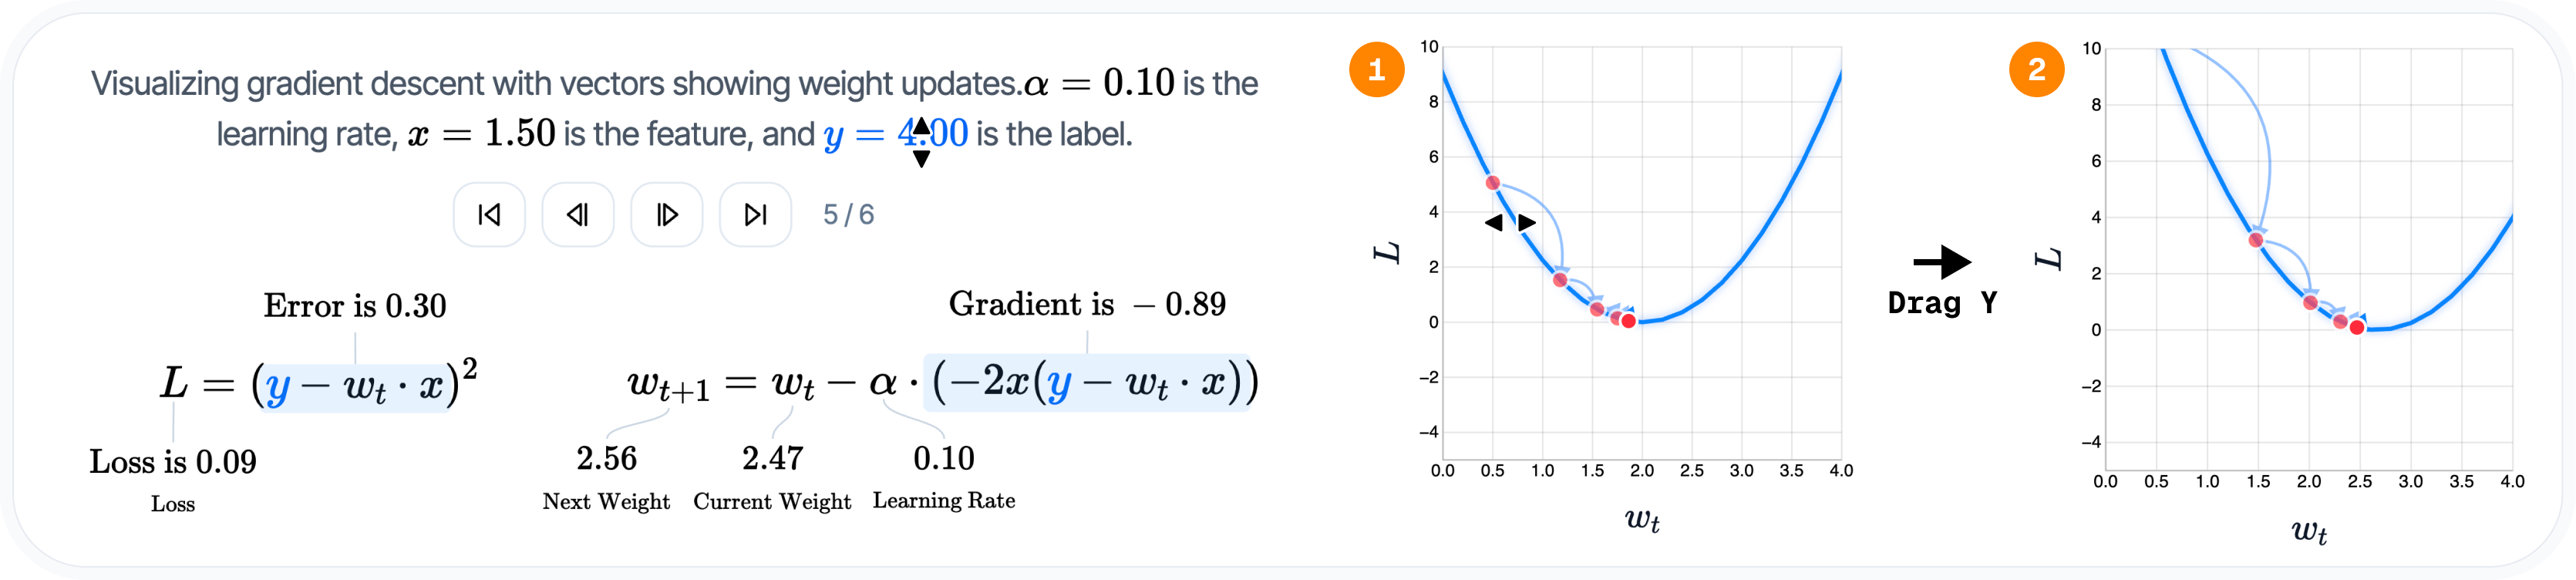
\includegraphics[width=\textwidth]{fig/system.png}
\caption{\textbf{Reactive propagation across steps and visualizations.} Dragging $y$ in the prose (1) triggers re-execution of the semantics function, updating all intermediate step values and shifting the visualization vectors (2) to reflect the new loss landscape. See Figure~\ref{fig:gradient-config} for the full configuration.}
\label{fig:system}
\end{figure*}
